% ========== 激活函数（8分） ==========
\chapter{激活函数（8分）}

\section{实现tanh激活函数的前向传播和反向传播（4分）}

\textbf{前向传播}

tanh 公式 $\tanh(x) = \frac{e^x - e^{-x}}{e^x + e^{-x}}$

\begin{lstlisting}[style=cleanpython]
    exp_x = np.exp(x)
    exp_neg_x = np.exp(-x)
    out = (exp_x - exp_neg_x) / (exp_x + exp_neg_x)
\end{lstlisting}

Jupyter Notebook 上的测试结果：

\begin{lstlisting}[style=cleanpython]
Testing tanh_forward function:
difference:  3.838674944915509e-09
\end{lstlisting}

\textbf{反向传播}

tanh 求导公式 $\tanh'(x) = 1 - \tanh^2(x)$

\begin{lstlisting}[style=cleanpython]
    tanh_x = cache
    dx = dout * (1 - tanh_x**2)
\end{lstlisting}

Jupyter Notebook 上的测试结果：

\begin{lstlisting}[style=cleanpython]
Testing tanh_backward function:
dx error:  1.0409584283255793e-10
\end{lstlisting}

\section{实现 sigmoid 激活函数的前向传播和反向传播（4分）}

\textbf{前向传播}

Sigmoid公式为 $\sigma(x) = \frac{1}{1 + e^{-x}}$

\begin{lstlisting}[style=cleanpython]
    out = 1 / (1 + np.exp(-x))
\end{lstlisting}

Jupyter Notebook 上的测试结果：

\begin{lstlisting}[style=cleanpython]
Testing sigmoid_forward function:
difference:  5.296529106595102e-09
\end{lstlisting}

\textbf{反向传播}

Sigmoid求导公式为 $\sigma'(x) = \sigma(x) \cdot (1 - \sigma(x))$

\begin{lstlisting}[style=cleanpython]
    sigmoid_x = cache
    dx = dout * sigmoid_x * (1 - sigmoid_x)
\end{lstlisting}

Jupyter Notebook 上的测试结果：

\begin{lstlisting}[style=cleanpython]
Testing sigmoid_backward function:
dx error:  3.446520386706568e-11
\end{lstlisting}

% ========== 全连接神经网络（15分） ==========
\chapter{全连接神经网络（15分）}

\section{实现 affine layer 的前向传播和反向传播（3分）}

\textbf{前向传播}

全连接层的数学表达式为 $Z = XW + b$，其中 $X$ 是输入矩阵，$W$ 是权重矩阵，$b$ 是偏置向量。

\begin{lstlisting}[style=cleanpython]
x_row = x.reshape(x.shape[0], -1)
out = x_row.dot(w) + b
\end{lstlisting}

Jupyter Notebook 上的测试结果：

\begin{lstlisting}[style=cleanpython]
Testing affine_forward function:
difference:  9.769849468192957e-10
\end{lstlisting}

\textbf{反向传播}

梯度计算公式：
$$\frac{\partial L}{\partial W} = X^T \cdot \frac{\partial L}{\partial Z},\quad
\frac{\partial L}{\partial b} = \sum_{i=1}^{N} \frac{\partial L}{\partial Z_i},\quad
\frac{\partial L}{\partial X} = \frac{\partial L}{\partial Z} \cdot W^T$$

\begin{lstlisting}[style=cleanpython]
x_row = x.reshape(x.shape[0], -1)
dx = dout.dot(w.T).reshape(x.shape)
dw = x_row.T.dot(dout)
db = np.sum(dout, axis=0)
\end{lstlisting}

Jupyter Notebook 上的测试结果：

\begin{lstlisting}[style=cleanpython]
Testing affine_backward function:
dx error:  5.399100368651805e-11
dw error:  9.904211865398145e-11
db error:  2.4122867568119087e-11
\end{lstlisting}

\section{实现 ReLU 激活函数的前向传播和反向传播，并在 Jupyter Notebook 上回答问题 1（3分）}

\textbf{前向传播}

ReLU 的数学表达式为 $f(x) = \max(0, x)$。

\begin{lstlisting}[style=cleanpython]
out = np.maximum(0, x)
\end{lstlisting}

Jupyter Notebook 上的测试结果：

\begin{lstlisting}[style=cleanpython]
Testing relu_forward function:
difference:  4.999999798022158e-08
\end{lstlisting}

\textbf{反向传播}

ReLU 的导数：
$$f'(x) = \begin{cases}
1, & \text{if } x > 0 \\
0, & \text{if } x \leq 0
\end{cases}$$

\begin{lstlisting}[style=cleanpython]
dx = dout.copy()
dx[x <= 0] = 0
\end{lstlisting}

Jupyter Notebook 上的测试结果：

\begin{lstlisting}[style=cleanpython]
Testing relu_backward function:
dx error:  3.2756349136310288e-12
\end{lstlisting}

问题已经在Jupyter Notebook中回答。

\section{利用你实现的 affine layer 和 ReLU 激活函数构建一个两层的全连接神经网络（3分）}

本次实验实现了一个两层全连接神经网络，其架构为 \texttt{affine - relu - affine - softmax}，包含第一层（affine+ReLU）、第二层（affine）和softmax交叉熵损失。

\textbf{初始化参数}

\begin{lstlisting}[style=cleanpython]
self.params["W1"] = weight_scale * np.random.randn(input_dim, hidden_dim)
self.params["b1"] = np.zeros(hidden_dim)
self.params["W2"] = weight_scale * np.random.randn(hidden_dim, num_classes)
self.params["b2"] = np.zeros(num_classes)
\end{lstlisting}

权重从高斯分布 $\mathcal{N}(0, \text{weight\_scale})$ 采样，偏置初始化为0。

\textbf{前向传播}

\begin{lstlisting}[style=cleanpython]
hidden, cache_hidden = affine_relu_forward(X, self.params["W1"], self.params["b1"])
scores, cache_scores = affine_forward(hidden, self.params["W2"], self.params["b2"])
\end{lstlisting}

\textbf{损失计算和反向传播}

\begin{lstlisting}[style=cleanpython]
loss, dscores = softmax_loss(scores, y)
loss += 0.5 * self.reg * (np.sum(self.params["W1"] ** 2)
                         + np.sum(self.params["W2"] ** 2))

dhidden, dW2, db2 = affine_backward(dscores, cache_scores)
dX, dW1, db1 = affine_relu_backward(dhidden, cache_hidden)

grads["W2"] = dW2 + self.reg * self.params["W2"]
grads["b2"] = db2
grads["W1"] = dW1 + self.reg * self.params["W1"]
grads["b1"] = db1
\end{lstlisting}

Jupyter Notebook 上的梯度检查结果：

\begin{lstlisting}[style=cleanpython]
Running numeric gradient check with reg =  0.0
W1 relative error: 1.83e-08
W2 relative error: 3.12e-10
b1 relative error: 9.83e-09
b2 relative error: 4.33e-10
Running numeric gradient check with reg =  0.7
W1 relative error: 2.53e-07
W2 relative error: 2.85e-08
b1 relative error: 1.56e-08
b2 relative error: 7.76e-10
\end{lstlisting}

\section{训练你实现的两层全连接神经网络，使测试结果的准确率达到 50\% 以上（3分）}

为了让两层网络具备足够的拟合能力，本次训练将隐藏层维度设置为 1000，并采用较小的学习率 1e-3；这样既能保持优化过程稳定，也更容易在验证集上超过 50\% 的准确率。

\begin{lstlisting}[style=cleanpython]
model = TwoLayerNet()
solver = Solver(model, data,
                print_every=100, num_epochs=10, batch_size=200,
                update_rule='sgd',
                optim_config={'learning_rate': 1e-3},
                lr_decay=0.95,
                verbose=True)
solver.train()
\end{lstlisting}

训练过程
\begin{lstlisting}[style=cleanpython]
(Iteration 1 / 2450) loss: 2.305965
(Epoch 0 / 10) train acc: 0.114000; val_acc: 0.096000
(Iteration 101 / 2450) loss: 1.856329
(Iteration 201 / 2450) loss: 1.598619
(Epoch 1 / 10) train acc: 0.407000; val_acc: 0.416000
(Iteration 301 / 2450) loss: 1.548536
(Iteration 401 / 2450) loss: 1.661861
(Epoch 2 / 10) train acc: 0.491000; val_acc: 0.462000
(Iteration 501 / 2450) loss: 1.452303
(Iteration 601 / 2450) loss: 1.665413
(Iteration 701 / 2450) loss: 1.295910
(Epoch 3 / 10) train acc: 0.485000; val_acc: 0.461000
(Iteration 801 / 2450) loss: 1.393038
(Iteration 901 / 2450) loss: 1.395341
(Epoch 4 / 10) train acc: 0.533000; val_acc: 0.499000
(Iteration 1001 / 2450) loss: 1.449278
(Iteration 1101 / 2450) loss: 1.276145
(Iteration 1201 / 2450) loss: 1.207275
(Epoch 5 / 10) train acc: 0.520000; val_acc: 0.516000
(Iteration 1301 / 2450) loss: 1.339874
(Iteration 1401 / 2450) loss: 1.430487
(Epoch 6 / 10) train acc: 0.534000; val_acc: 0.507000
(Iteration 1501 / 2450) loss: 1.364778
(Iteration 1601 / 2450) loss: 1.167146
(Iteration 1701 / 2450) loss: 1.362156
...
(Iteration 2301 / 2450) loss: 1.229667
(Iteration 2401 / 2450) loss: 1.104043
(Epoch 10 / 10) train acc: 0.597000; val_acc: 0.518000
Best val acc:  0.518
\end{lstlisting}

运行截图：
\begin{figure}[htbp]
\centering
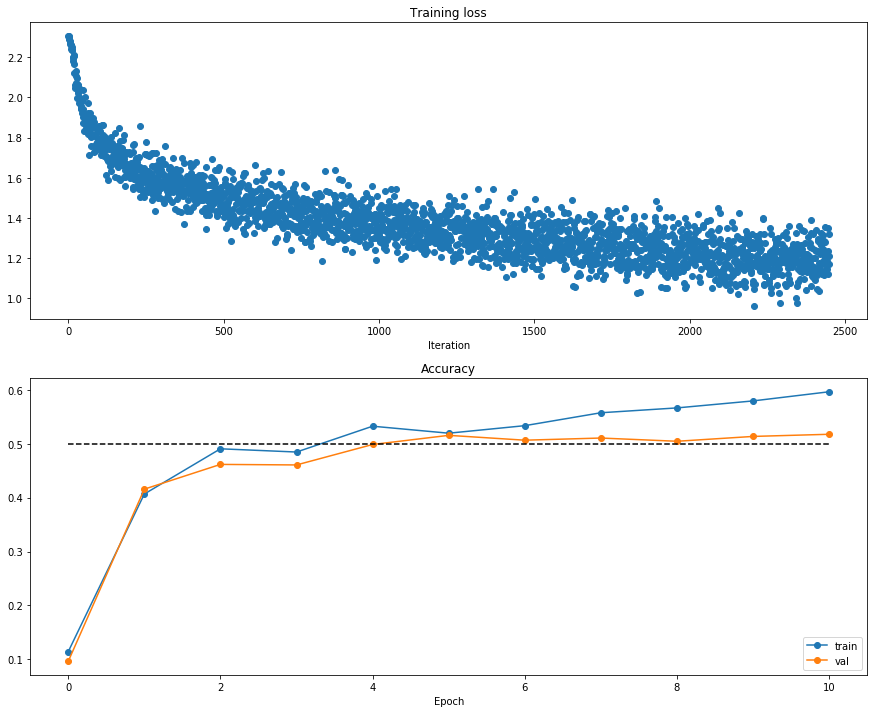
\includegraphics[width=0.8\textwidth]{image/Solver.png}
\end{figure}

\section{构建多层的全连接网络，满足 \texttt{FullyConnectedNets.ipynb} 中的测试要求（3分）}

实现了一个具有任意数量隐藏层的全连接神经网络，支持dropout正则化，并为批量归一化和层归一化做了准备。

\textbf{网络架构}

\begin{center}
\texttt{\{affine - [batch/layer norm] - relu - [dropout]\} $\times$ (L - 1) - affine - softmax}
\end{center}

其中 L 是网络的总层数，batch/layer norm和dropout是可选的。

\textbf{参数初始化}

\begin{lstlisting}[style=cleanpython]
layer_dims = [input_dim] + list(hidden_dims) + [num_classes]
for i in range(1, self.num_layers + 1):
    self.params[f"W{i}"] = weight_scale * np.random.randn(
        layer_dims[i - 1], layer_dims[i])
    self.params[f"b{i}"] = np.zeros(layer_dims[i])
    if i < self.num_layers and self.normalization in {"batchnorm", "layernorm"}:
        self.params[f"gamma{i}"] = np.ones(layer_dims[i])
        self.params[f"beta{i}"] = np.zeros(layer_dims[i])
\end{lstlisting}

权重从高斯分布 $\mathcal{N}(0, \text{weight\_scale})$ 采样，偏置初始化为0。对于归一化层，gamma初始化为1，beta初始化为0。

\textbf{前向传播}

\begin{lstlisting}[style=cleanpython]
caches = []
out = X
for i in range(1, self.num_layers):
    W = self.params[f"W{i}"]
    b = self.params[f"b{i}"]
    out, fc_cache = affine_forward(out, W, b)

    norm_cache = None
    if self.normalization == "batchnorm":
        gamma = self.params[f"gamma{i}"]
        beta = self.params[f"beta{i}"]
        out, norm_cache = batchnorm_forward(out, gamma, beta, self.bn_params[i - 1])
    elif self.normalization == "layernorm":
        gamma = self.params[f"gamma{i}"]
        beta = self.params[f"beta{i}"]
        out, norm_cache = layernorm_forward(out, gamma, beta, self.bn_params[i - 1])

    out, relu_cache = relu_forward(out)
    dropout_cache = None
    if self.use_dropout:
        out, dropout_cache = dropout_forward(out, self.dropout_param)
    caches.append((fc_cache, norm_cache, relu_cache, dropout_cache))

scores, final_cache = affine_forward(
    out, self.params[f"W{self.num_layers}"], self.params[f"b{self.num_layers}"])
\end{lstlisting}

\textbf{反向传播}

\begin{lstlisting}[style=cleanpython]
loss, dscores = softmax_loss(scores, y)
for i in range(1, self.num_layers + 1):
    W = self.params[f"W{i}"]
    loss += 0.5 * self.reg * np.sum(W ** 2)

dx, dW, db = affine_backward(dscores, final_cache)
grads[f"W{self.num_layers}"] = dW + self.reg * self.params[f"W{self.num_layers}"]
grads[f"b{self.num_layers}"] = db

for i in range(self.num_layers - 1, 0, -1):
    fc_cache, norm_cache, relu_cache, dropout_cache = caches[i - 1]
    if self.use_dropout:
        dx = dropout_backward(dx, dropout_cache)
    dx = relu_backward(dx, relu_cache)
    if self.normalization == "batchnorm":
        dx, dgamma, dbeta = batchnorm_backward(dx, norm_cache)
        grads[f"gamma{i}"] = dgamma
        grads[f"beta{i}"] = dbeta
    elif self.normalization == "layernorm":
        dx, dgamma, dbeta = layernorm_backward(dx, norm_cache)
        grads[f"gamma{i}"] = dgamma
        grads[f"beta{i}"] = dbeta
    dx, dW, db = affine_backward(dx, fc_cache)
    grads[f"W{i}"] = dW + self.reg * self.params[f"W{i}"]
    grads[f"b{i}"] = db
\end{lstlisting}

\textbf{梯度检查结果}

初始损失看起来合理，梯度检查误差在 1e-7 或更小：

Jupyter Notebook 上的梯度检查结果：

\begin{lstlisting}[style=cleanpython]
Running check with reg =  0
Initial loss:  2.3004790897684924
W1 relative error: 1.48e-07
W2 relative error: 2.21e-05
W3 relative error: 3.53e-07
b1 relative error: 5.38e-09
b2 relative error: 2.09e-09
b3 relative error: 5.80e-11
Running check with reg =  3.14
Initial loss:  7.052114776533016
W1 relative error: 3.90e-09
W2 relative error: 6.87e-08
W3 relative error: 2.13e-08
b1 relative error: 1.48e-08
b2 relative error: 1.72e-09
b3 relative error: 1.57e-10
\end{lstlisting}

\textbf{三层网络过拟合测试}

对一个包含50张图像的小数据集，调整学习率和权重初始化尺度，在20个训练周期内达到100\%的训练准确率：

\begin{lstlisting}[style=cleanpython]
weight_scale = 5e-2
learning_rate = 1e-3
\end{lstlisting}

训练过程
\begin{lstlisting}[style=cleanpython]
(Iteration 1 / 40) loss: 29.590974
(Epoch 0 / 20) train acc: 0.260000; val_acc: 0.132000
(Epoch 1 / 20) train acc: 0.340000; val_acc: 0.087000
(Epoch 2 / 20) train acc: 0.540000; val_acc: 0.124000
(Epoch 3 / 20) train acc: 0.600000; val_acc: 0.147000
(Epoch 4 / 20) train acc: 0.800000; val_acc: 0.150000
(Epoch 5 / 20) train acc: 0.820000; val_acc: 0.139000
(Iteration 11 / 40) loss: 2.673592
(Epoch 6 / 20) train acc: 0.940000; val_acc: 0.136000
(Epoch 7 / 20) train acc: 0.980000; val_acc: 0.134000
(Epoch 8 / 20) train acc: 1.000000; val_acc: 0.132000
(Epoch 9 / 20) train acc: 1.000000; val_acc: 0.133000
(Epoch 10 / 20) train acc: 1.000000; val_acc: 0.132000
(Iteration 21 / 40) loss: 0.001749
(Epoch 11 / 20) train acc: 1.000000; val_acc: 0.133000
(Epoch 12 / 20) train acc: 1.000000; val_acc: 0.132000
(Epoch 13 / 20) train acc: 1.000000; val_acc: 0.131000
(Epoch 14 / 20) train acc: 1.000000; val_acc: 0.130000
(Epoch 15 / 20) train acc: 1.000000; val_acc: 0.130000
(Iteration 31 / 40) loss: 0.002012
(Epoch 16 / 20) train acc: 1.000000; val_acc: 0.132000
(Epoch 17 / 20) train acc: 1.000000; val_acc: 0.132000
(Epoch 18 / 20) train acc: 1.000000; val_acc: 0.132000
(Epoch 19 / 20) train acc: 1.000000; val_acc: 0.131000
(Epoch 20 / 20) train acc: 1.000000; val_acc: 0.131000
\end{lstlisting}

训练损失图：

\begin{figure}[htbp]
\centering
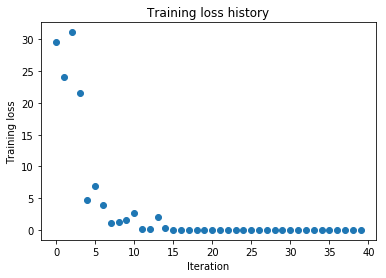
\includegraphics[width=0.8\textwidth]{image/Multilayer network 1.png}
\end{figure}

\textbf{五层网络过拟合测试}

\begin{lstlisting}[style=cleanpython]
learning_rate = 1e-2
weight_scale = 5e-2
\end{lstlisting}

训练过程：
\begin{lstlisting}[style=cleanpython]
(Iteration 1 / 40) loss: 4.305139
(Epoch 0 / 20) train acc: 0.160000; val_acc: 0.107000
(Epoch 1 / 20) train acc: 0.180000; val_acc: 0.105000
(Epoch 2 / 20) train acc: 0.460000; val_acc: 0.116000
(Epoch 3 / 20) train acc: 0.640000; val_acc: 0.123000
(Epoch 4 / 20) train acc: 0.740000; val_acc: 0.122000
(Epoch 5 / 20) train acc: 0.880000; val_acc: 0.138000
(Iteration 11 / 40) loss: 0.545579
(Epoch 6 / 20) train acc: 0.960000; val_acc: 0.140000
(Epoch 7 / 20) train acc: 0.960000; val_acc: 0.139000
(Epoch 8 / 20) train acc: 0.980000; val_acc: 0.139000
(Epoch 9 / 20) train acc: 1.000000; val_acc: 0.143000
(Epoch 10 / 20) train acc: 1.000000; val_acc: 0.152000
(Iteration 21 / 40) loss: 0.081050
(Epoch 11 / 20) train acc: 1.000000; val_acc: 0.147000
(Epoch 12 / 20) train acc: 1.000000; val_acc: 0.155000
(Epoch 13 / 20) train acc: 1.000000; val_acc: 0.150000
(Epoch 14 / 20) train acc: 1.000000; val_acc: 0.145000
(Epoch 15 / 20) train acc: 1.000000; val_acc: 0.150000
(Iteration 31 / 40) loss: 0.050216
(Epoch 16 / 20) train acc: 1.000000; val_acc: 0.150000
(Epoch 17 / 20) train acc: 1.000000; val_acc: 0.149000
(Epoch 18 / 20) train acc: 1.000000; val_acc: 0.151000
(Epoch 19 / 20) train acc: 1.000000; val_acc: 0.152000
(Epoch 20 / 20) train acc: 1.000000; val_acc: 0.152000
\end{lstlisting}

训练损失图：

\begin{figure}[htbp]
\centering
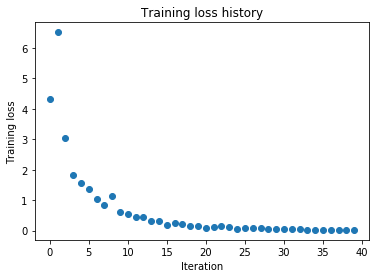
\includegraphics[width=0.8\textwidth]{image/Multilayer network 2.png}
\end{figure}

% ========== 归一化（10分） ==========
\chapter{归一化（10分）}

\section{实现 batch normalization 的前向传播和反向传播（3分）}

在文件 \texttt{annp/layers.py} 中实现批量归一化。

\textbf{前向传播（训练模式）}

当 \texttt{mode} 为 \texttt{"train"} 时，计算批次均值与方差，对数据进行标准化，再进行缩放和平移，最后更新运行时统计量。

\begin{lstlisting}[style=cleanpython]
if mode == "train":
    sample_mean = np.mean(x, axis=0)
    sample_var = np.var(x, axis=0)
    x_hat = (x - sample_mean) / np.sqrt(sample_var + eps)
    out = gamma * x_hat + beta
    running_mean = momentum * running_mean + (1 - momentum) * sample_mean
    running_var = momentum * running_var + (1 - momentum) * sample_var
    cache = (x_hat, gamma, sample_var, eps)
\end{lstlisting}

Jupyter Notebook 上的测试结果：

\begin{lstlisting}[style=cleanpython]
After batch normalization (gamma=1, beta=0)
  means:  [5.32907052e-17 7.04991621e-17 1.85962357e-17]
  stds:   [0.99999999 1.         1.        ]
After batch normalization (gamma= [1. 2. 3.] , beta= [11. 12. 13.] )
  means:  [11. 12. 13.]
  stds:   [0.99999999 1.99999999 2.99999999]
\end{lstlisting}

\textbf{前向传播（测试模式）}

当 \texttt{mode} 为 \texttt{"test"} 时，使用运行时统计量进行标准化：

\begin{lstlisting}[style=cleanpython]
elif mode == "test":
    x_hat = (x - running_mean) / np.sqrt(running_var + eps)
    out = gamma * x_hat + beta
\end{lstlisting}

测试结果：
\begin{lstlisting}[style=cleanpython]
After batch normalization (test-time):
  means:  [-0.03927354 -0.04349152 -0.10452688]
  stds:   [1.01531428 1.01238373 0.97819988]
\end{lstlisting}


\textbf{反向传播}

\begin{lstlisting}[style=cleanpython]
    x_hat, gamma, sample_var, eps = cache
    N = dout.shape[0]

    dbeta = np.sum(dout, axis=0)
    dgamma = np.sum(dout * x_hat, axis=0)

    inv_std = 1.0 / np.sqrt(sample_var + eps)
    dx = (1.0 / N) * gamma * inv_std * (
      N * dout - np.sum(dout, axis=0) - x_hat * np.sum(dout * x_hat, axis=0)
    )
\end{lstlisting}

Jupyter Notebook 上的测试结果：

\begin{lstlisting}[style=cleanpython]
dx error:  1.7029243421054735e-09
dgamma error:  7.420414216247087e-13
dbeta error:  2.8795057655839487e-12
\end{lstlisting}

\section{修改你之前实现的全连接神经网络，添加 batch normalization，回答问题 1（3分）}

\textbf{前向传播修改}

当 \texttt{normalization} 参数设置为 \texttt{'batchnorm'} 时，在每个ReLU非线性激活层之前插入批量归一化层：

\begin{lstlisting}[style=cleanpython]
if self.normalization == 'batchnorm':
    gamma = self.params[f'gamma{i}']
    beta = self.params[f'beta{i}']
    x, fc_cache = affine_forward(x, W, b)
    x, norm_cache = batchnorm_forward(x, gamma, beta, self.bn_params[i - 1])
    x, relu_cache = relu_forward(x)
    cache = (fc_cache, norm_cache, relu_cache)
else:
    x, cache = affine_relu_forward(x, W, b)
\end{lstlisting}

\textbf{反向传播修改}

\begin{lstlisting}[style=cleanpython]
if self.normalization == 'batchnorm':
    fc_cache, norm_cache, relu_cache = caches[i]
    dx = relu_backward(dx, relu_cache)
    dx, dgamma, dbeta = batchnorm_backward(dx, norm_cache)
    dx, dw, db = affine_backward(dx, fc_cache)
    grads[f'gamma{i}'] = dgamma
    grads[f'beta{i}'] = dbeta
else:
    dx, dw, db = affine_relu_backward(dx, caches[i])
\end{lstlisting}

\textbf{可视化运行结果}

\begin{figure}[htbp]
\centering
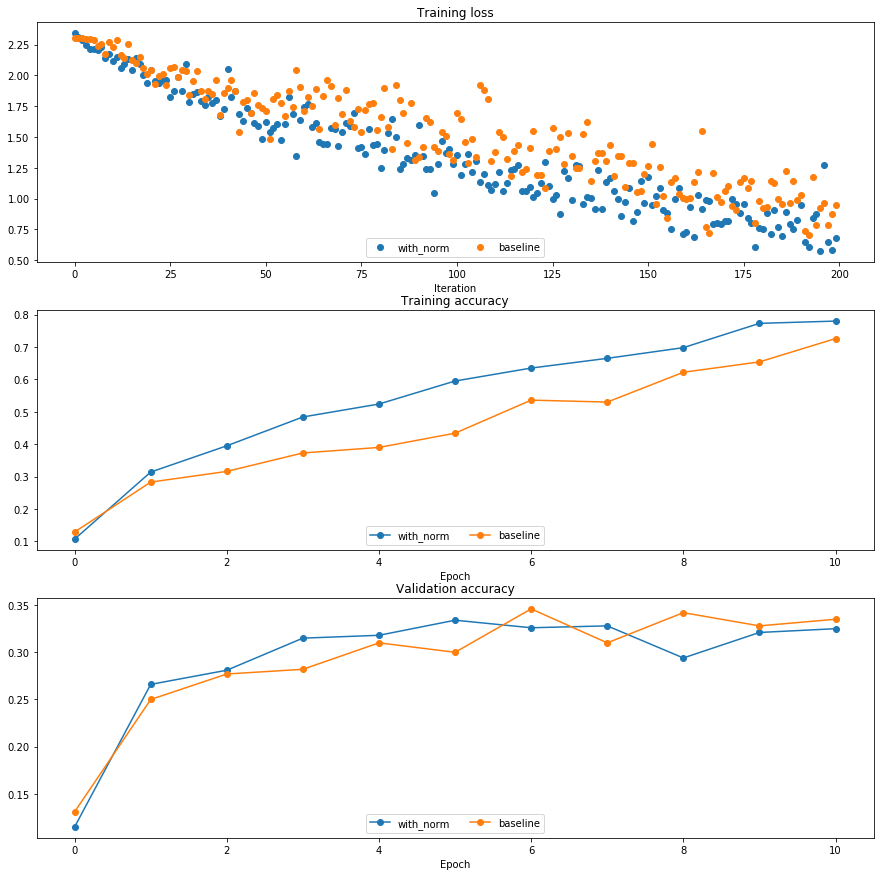
\includegraphics[width=0.8\textwidth]{image/Batchnorm for deep networks.png}
\end{figure}

\begin{figure}[htbp]
\centering
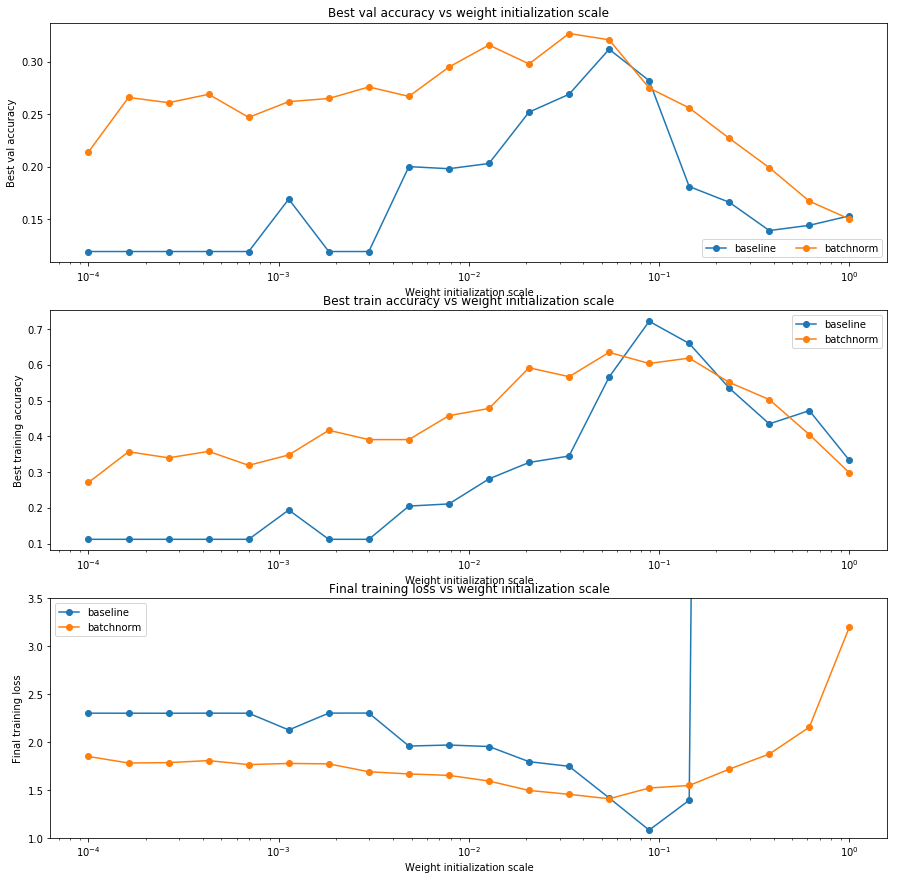
\includegraphics[width=0.8\textwidth]{image/Batch normalization and initialization.png}
\end{figure}

\textbf{回答问题一}

\paragraph{描述实验结果：}实验在 $10^{-4}$ 至 $10^0$ 范围内取了 20 个权重初始化尺度，分别训练有/无 BatchNorm 的 8 层全连接网络，并观察最佳训练准确率、最佳验证准确率和最终训练损失随初始化尺度的变化。根据图中的曲线，无 BatchNorm 模型的验证准确率随初始化尺度变化更明显，且在较大尺度下训练损失容易升高；有 BatchNorm 模型在大多数初始化尺度下表现更稳定，训练损失整体也更平缓。

\paragraph{不同影响：}权重初始化尺度对有无 BatchNorm 的模型影响较明显。无 BatchNorm 模型在较小或较大尺度下都更容易出现训练不稳定的情况；有 BatchNorm 模型则对初始化尺度更不敏感，在图中的大部分区间里都保持了相对平稳的训练过程和更好的验证表现。

\paragraph{原因：}无 BatchNorm 时，权重尺度的变化会直接影响各层激活值的量级，进而影响优化稳定性。BatchNorm 对每层激活值做标准化（零均值、单位方差），使各层输入分布与权重初始化尺度部分解耦；标准化后的输出再由可学习的 $\gamma, \beta$ 重新调节，因此网络通常对初始化选择没有那么敏感。

\section{探究 batch normalization 和 batch size 的关系，回答问题 2（2分）}

\begin{figure}[htbp]
\centering
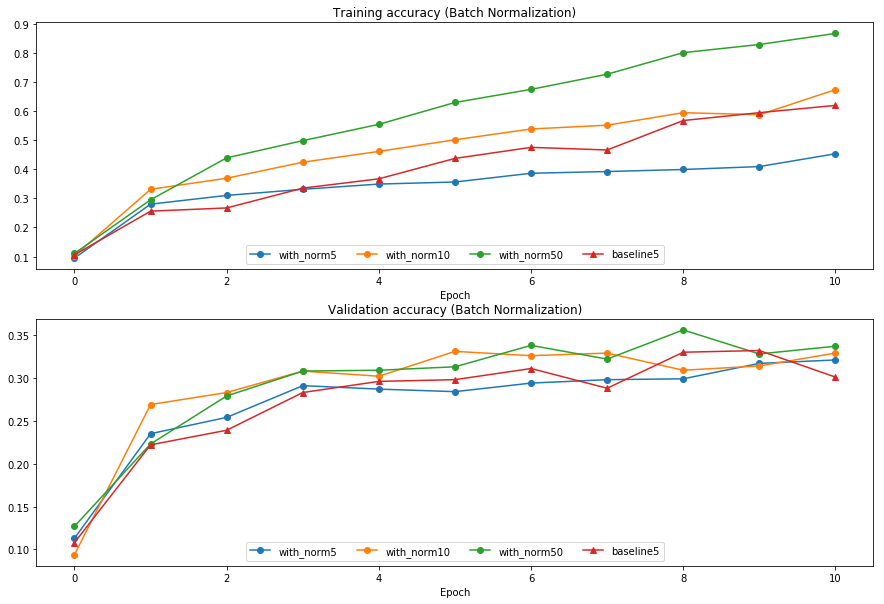
\includegraphics[width=0.8\textwidth]{image/Batch normalization and batch size.png}
\end{figure}

\textbf{实验结果：}

随着训练轮数（Epoch）增加，使用批量归一化（Batch Normalization）的模型（\texttt{with\_norm5}、\texttt{with\_norm10}、\texttt{with\_norm50}）在图中的训练准确率整体上高于 \texttt{baseline5}。从曲线形状看，\texttt{with\_norm50} 的训练准确率更高，\texttt{with\_norm10} 和 \texttt{with\_norm5} 也都比基线更平稳。

一开始，使用批量归一化的模型的验证准确率会有一定波动；在后续训练阶段，\texttt{with\_norm50} 和 \texttt{with\_norm10} 的表现通常更接近较优区域，而 \texttt{baseline5} 的验证准确率整体更低、波动也更明显。

\textbf{批量归一化与批量大小的关系：}

在这组实验设置下，较大的 batch size 往往对应更平滑的训练曲线和更高的准确率上限；但这一结论更适合表述为“在本实验中较大的 batch size 表现更好”，而不是对所有任务都成立的普遍规律。

\textbf{出现这种关系的原因：}

批量归一化会对神经网络各层的输入进行归一化。较大的批量通常能提供更稳定的均值和方差估计，因此归一化过程更平滑；较小的批量下，统计量波动会更明显，训练曲线也更容易抖动。

较大的批量大小往往会带来更一致的梯度更新，因此优化过程看起来更稳定。不过，这里观察到的提升应主要理解为“在当前实验设置下的经验现象”，不宜直接推广为一般性的理论结论。

\section{实现 layer normalization 的前向传播和反向传播，并将 layer normalization 添加到你之前实现的全连接神经网络中（1分）}

\textbf{在 \texttt{annp/layers.py} 中实现层归一化的前向传播}

与批量归一化不同，层归一化沿着特征维度计算均值和方差：

\begin{lstlisting}[style=cleanpython]
    sample_mean = np.mean(x, axis=1, keepdims=True)
    sample_var = np.var(x, axis=1, keepdims=True)
    x_hat = (x - sample_mean) / np.sqrt(sample_var + eps)
    out = gamma * x_hat + beta
    cache = (x_hat, gamma, sample_var, eps)
\end{lstlisting}

Jupyter Notebook 上的测试结果：

\begin{lstlisting}[style=cleanpython]
Before layer normalization:
  means:  [-59.06673243 -47.60782686 -43.31137368 -26.40991744]
  stds:   [10.07429373 28.39478981 35.28360729  4.01831507]

After layer normalization (gamma=1, beta=0)
  means:  [ 4.81096644e-16 -7.40148683e-17  2.22044605e-16 -5.92118946e-16]
  stds:   [0.99999995 0.99999999 1.         0.99999969]

After layer normalization (gamma= [3. 3. 3.] , beta= [5. 5. 5.] )
  means:  [5. 5. 5. 5.]
  stds:   [2.99999985 2.99999998 2.99999999 2.99999907]
\end{lstlisting}

\textbf{在 \texttt{annp/layers.py} 中实现层归一化的反向传播}

\begin{lstlisting}[style=cleanpython]
    x_hat, gamma, sample_var, eps = cache
    N, D = dout.shape

    dbeta = np.sum(dout, axis=0)
    dgamma = np.sum(dout * x_hat, axis=0)

    inv_std = 1.0 / np.sqrt(sample_var + eps)
    dx = (1.0 / D) * (gamma * inv_std) * (
      D * dout - np.sum(dout, axis=1, keepdims=True)
      - x_hat * np.sum(dout * x_hat, axis=1, keepdims=True)
    )
\end{lstlisting}

Jupyter Notebook 上的测试结果：

\begin{lstlisting}[style=cleanpython]
dx error:  1.4336160411201157e-09
dgamma error:  4.519489546032799e-12
dbeta error:  2.276445013433725e-12
\end{lstlisting}

\textbf{修改 \texttt{fc\_net.py} 添加层归一化}

\texttt{layernorm\_forward} 和 \texttt{layernorm\_backward} 已在 \texttt{annp/layers.py} 中实现，\texttt{fc\_net.py} 只需要在前向与反向传播中直接调用它们。

在网络中按如下方式使用：

\begin{lstlisting}[style=cleanpython]
elif self.normalization == "layernorm":
    gamma = self.params[f"gamma{i}"]
    beta = self.params[f"beta{i}"]
    out, norm_cache = layernorm_forward(out, gamma, beta, self.bn_params[i - 1])
\end{lstlisting}

\section{探究 layer normalization 和 batch size 的关系，回答问题 3（1分）}

\begin{figure}[htbp]
\centering
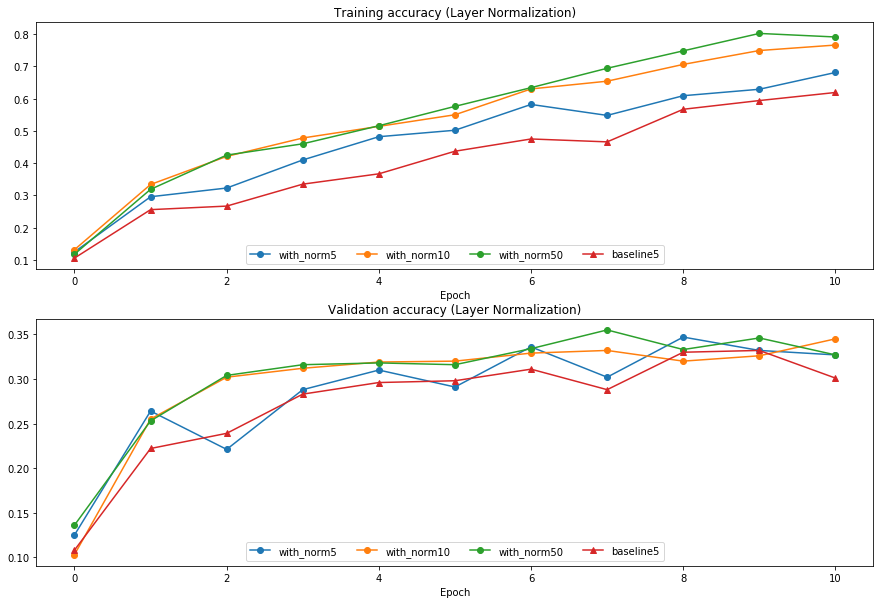
\includegraphics[width=0.8\textwidth]{image/Layer Normalization and batch size.png}
\end{figure}

\textbf{回答问题3}

在这组选项里，更贴近当前实验结果的解释是“特征维度非常小”。

层归一化是对单个样本的所有特征维度计算均值和方差进行标准化。当特征维度 $D$ 非常小时（例如 $D < 5$），仅凭少量特征值估计出的均值和方差极不稳定，标准化后几乎抹平了各特征之间的相对差异，破坏了数据原有的信息结构。此时归一化引入的噪声反而超过其稳定训练的作用，导致模型性能下降。

非常深的网络不应作为主要答案：层归一化确实常用于深层网络，但“网络很深”本身并不是导致性能下降的直接原因。

正则化项过大也不应作为主要答案：正则化强度会影响训练，但它与层归一化问题的直接关系并不强，通常不是解释该现象的首要因素。

% ========== CNN（32分） ==========
\chapter{CNN（32分）}

\section{实现 CNN 的前向传播和反向传播（5分）}

修改 \texttt{conv\_forward\_naive} 和 \texttt{conv\_backward\_naive}。

\textbf{前向传播}

\begin{lstlisting}[style=cleanpython]
N, C, H, W = x.shape
F, _, HH, WW = w.shape
stride = conv_param['stride']
pad = conv_param['pad']
H_out = 1 + (H + 2 * pad - HH) // stride
W_out = 1 + (W + 2 * pad - WW) // stride
out = np.zeros((N, F, H_out, W_out))
x_padded = np.pad(x, ((0, 0), (0, 0), (pad, pad), (pad, pad)), mode='constant')

for n in range(N):
    for f in range(F):
        for h_out in range(H_out):
            for w_out in range(W_out):
                h_start = h_out * stride
                w_start = w_out * stride
                x_window = x_padded[n, :, h_start:h_start+HH, w_start:w_start+WW]
                out[n, f, h_out, w_out] = np.sum(x_window * w[f]) + b[f]
\end{lstlisting}

Jupyter Notebook 上的测试结果：

\begin{lstlisting}[style=cleanpython]
Testing conv_forward_naive
difference:  2.2121476417505994e-08
\end{lstlisting}

卷积操作的直观展示——灰度转换与边缘检测：

\begin{figure}[htbp]
\centering
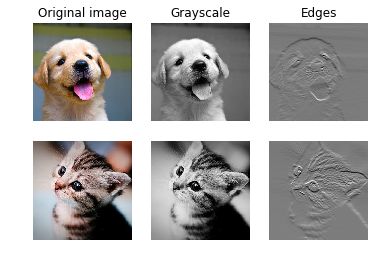
\includegraphics[width=0.8\textwidth]{image/Aside Image processing via convolutions.png}
\caption{卷积操作示意：原始图像 → 灰度转换 / 边缘检测}
\end{figure}

\textbf{反向传播}

\begin{lstlisting}[style=cleanpython]
    x, w, b, conv_param = cache
    stride = conv_param['stride']
    pad = conv_param['pad']
    N, C, H, W = x.shape
    F, _, HH, WW = w.shape
    _, _, H_out, W_out = dout.shape
    dx = np.zeros_like(x)
    dw = np.zeros_like(w)
    db = np.zeros_like(b)
    x_padded = np.pad(x, ((0, 0), (0, 0), (pad, pad), (pad, pad)), mode='constant')
    dx_padded = np.zeros_like(x_padded)

    for f in range(F):
        db[f] = np.sum(dout[:, f, :, :])

    for n in range(N):
        for f in range(F):
            for h_out in range(H_out):
                for w_out in range(W_out):
                    h_start = h_out * stride
                    w_start = w_out * stride
                    x_window = x_padded[n, :, h_start:h_start+HH, w_start:w_start+WW]
                    dw[f] += x_window * dout[n, f, h_out, w_out]
                    dx_padded[n, :, h_start:h_start+HH, w_start:w_start+WW] += \
                        w[f] * dout[n, f, h_out, w_out]

    dx = dx_padded[:, :, pad:pad+H, pad:pad+W]
\end{lstlisting}

Jupyter Notebook 上的测试结果：

\begin{lstlisting}[style=cleanpython]
Testing conv_backward_naive function
dx error:  1.159803161159293e-08
dw error:  2.2471264748452487e-10
db error:  3.37264006649648e-11
\end{lstlisting}

\section{实现 max pooling 的前向传播和反向传播（5分）}

\textbf{前向传播}

\begin{lstlisting}[style=cleanpython]
    N, C, H, W = x.shape
    pool_height = pool_param['pool_height']
    pool_width = pool_param['pool_width']
    stride = pool_param['stride']
    H_out = 1 + (H - pool_height) // stride
    W_out = 1 + (W - pool_width) // stride
    out = np.zeros((N, C, H_out, W_out))

    for n in range(N):
        for c in range(C):
            for h_out in range(H_out):
                for w_out in range(W_out):
                    h_start = h_out * stride
                    w_start = w_out * stride
                    pool_window = x[n, c, h_start:h_start+pool_height, w_start:w_start+pool_width]
                    out[n, c, h_out, w_out] = np.max(pool_window)

    cache = (x, pool_param)
\end{lstlisting}

Jupyter Notebook 上的测试结果：

\begin{lstlisting}[style=cleanpython]
Testing max_pool_forward_naive function:
difference:  4.1666665157267834e-08
\end{lstlisting}

\textbf{反向传播}

\begin{lstlisting}[style=cleanpython]
    x, pool_param = cache
    N, C, H, W = x.shape
    pool_height = pool_param['pool_height']
    pool_width = pool_param['pool_width']
    stride = pool_param['stride']
    _, _, H_out, W_out = dout.shape
    dx = np.zeros_like(x)

    for n in range(N):
        for c in range(C):
            for h_out in range(H_out):
                for w_out in range(W_out):
                    h_start = h_out * stride
                    w_start = w_out * stride
                    pool_window = x[n, c, h_start:h_start+pool_height, w_start:w_start+pool_width]
                    max_idx = np.argmax(pool_window.flatten())
                    max_i, max_j = np.unravel_index(max_idx, (pool_height, pool_width))
                    dx[n, c, h_start + max_i, w_start + max_j] += dout[n, c, h_out, w_out]
\end{lstlisting}

Jupyter Notebook 上的测试结果：

\begin{lstlisting}[style=cleanpython]
Testing max_pool_backward_naive function:
dx error:  3.27562514223145e-12
\end{lstlisting}

\section{实现 avg pooling 的前向传播和反向传播（5分）}

\textbf{前向传播}

\begin{lstlisting}[style=cleanpython]
    N, C, H, W = x.shape
    pool_height = pool_param['pool_height']
    pool_width = pool_param['pool_width']
    stride = pool_param['stride']
    H_out = 1 + (H - pool_height) // stride
    W_out = 1 + (W - pool_width) // stride
    out = np.zeros((N, C, H_out, W_out))

    for n in range(N):
        for c in range(C):
            for h_out in range(H_out):
                for w_out in range(W_out):
                    h_start = h_out * stride
                    w_start = w_out * stride
                    pool_window = x[n, c, h_start:h_start+pool_height, w_start:w_start+pool_width]
                    out[n, c, h_out, w_out] = np.mean(pool_window)
\end{lstlisting}

Jupyter Notebook 上的测试结果：

\begin{lstlisting}[style=cleanpython]
Testing avg_pool_forward_naive function:
difference:  1.8000003183688645e-07
\end{lstlisting}

\textbf{反向传播}

\begin{lstlisting}[style=cleanpython]
    x, pool_param = cache
    N, C, H, W = x.shape
    pool_height = pool_param['pool_height']
    pool_width = pool_param['pool_width']
    stride = pool_param['stride']
    _, _, H_out, W_out = dout.shape
    dx = np.zeros_like(x)

    for n in range(N):
        for c in range(C):
            for h_out in range(H_out):
                for w_out in range(W_out):
                    h_start = h_out * stride
                    w_start = w_out * stride
                    dx[n, c, h_start:h_start+pool_height, w_start:w_start+pool_width] += \
                        dout[n, c, h_out, w_out] / (pool_height * pool_width)
\end{lstlisting}

Jupyter Notebook 上的测试结果：

\begin{lstlisting}[style=cleanpython]
Testing avg_pool_backward_naive function:
dx error:  2.5480064605057958e-11
\end{lstlisting}

\section{实现一个三层卷积神经网络（5分）}

架构为 \texttt{conv - relu - 2x2 pool - affine - relu - affine - softmax}，包含一个卷积层、两个全连接层、ReLU激活函数和池化层。

\textbf{初始化参数}

\begin{lstlisting}[style=cleanpython]
C, H, W = input_dim
self.params["W1"] = weight_scale * np.random.randn(
    num_filters, C, filter_size, filter_size)
self.params["b1"] = np.zeros(num_filters)
conv_out_h = H // 2
conv_out_w = W // 2
affine_input_dim = num_filters * conv_out_h * conv_out_w
self.params["W2"] = weight_scale * np.random.randn(affine_input_dim, hidden_dim)
self.params["b2"] = np.zeros(hidden_dim)
self.params["W3"] = weight_scale * np.random.randn(hidden_dim, num_classes)
self.params["b3"] = np.zeros(num_classes)
\end{lstlisting}

\textbf{前向传播}

\begin{lstlisting}[style=cleanpython]
if self.pooling == "maxpool":
    a, cache_conv = conv_relu_maxpool_forward(X, W1, b1, conv_param, pool_param)
else:
    a, cache_conv = conv_relu_avgpool_forward(X, W1, b1, conv_param, pool_param)

a_flat = a.reshape(a.shape[0], -1)
hidden, cache_affine1 = affine_relu_forward(a_flat, W2, b2)
scores, cache_affine2 = affine_forward(hidden, W3, b3)
\end{lstlisting}

\textbf{反向传播}

\begin{lstlisting}[style=cleanpython]
loss, dscores = softmax_loss(scores, y)
loss += 0.5 * self.reg * (np.sum(W1 ** 2) + np.sum(W2 ** 2) + np.sum(W3 ** 2))

dhidden, dW3, db3 = affine_backward(dscores, cache_affine2)
da_flat, dW2, db2 = affine_relu_backward(dhidden, cache_affine1)
da = da_flat.reshape(a.shape)

if self.pooling == "maxpool":
    dx, dW1, db1 = conv_relu_maxpool_backward(da, cache_conv)
else:
    dx, dW1, db1 = conv_relu_avgpool_backward(da, cache_conv)

grads["W3"] = dW3 + self.reg * W3
grads["b3"] = db3
grads["W2"] = dW2 + self.reg * W2
grads["b2"] = db2
grads["W1"] = dW1 + self.reg * W1
grads["b1"] = db1
\end{lstlisting}

\textbf{运行结果}

过拟合小数据集训练后，损失、训练准确率和验证准确率显示出明显的过拟合：

\begin{figure}[htbp]
\centering
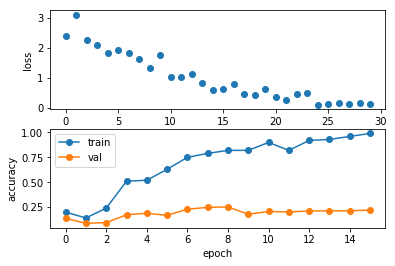
\includegraphics[width=0.8\textwidth]{image/Overfit small data.png}
\end{figure}

准确率：

\begin{lstlisting}[style=cleanpython]
Full data training accuracy: 0.4
Full data validation accuracy: 0.499
\end{lstlisting}

\begin{figure}[htbp]
\centering
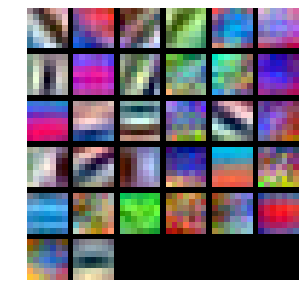
\includegraphics[width=0.8\textwidth]{image/Train the net.png}
\end{figure}

\section{实现 spatial batch normalization（5分）}

将卷积特征图先转置并重塑为 \lstinline|(-1, C)|，调用普通 batch normalization，再重塑回原始形状。

\textbf{前向传播}

\begin{lstlisting}[style=cleanpython]
N, C, H, W = x.shape
x_reshaped = x.transpose(0, 2, 3, 1).reshape(-1, C)
out, cache = batchnorm_forward(x_reshaped, gamma, beta, bn_param)
out = out.reshape(N, H, W, C).transpose(0, 3, 1, 2)
\end{lstlisting}

Jupyter Notebook 上的测试结果：

\begin{lstlisting}[style=cleanpython]
Before spatial batch normalization:
  Shape:  (2, 3, 4, 5)
  Means:  [9.33463814 8.90909116 9.11056338]
  Stds:  [3.61447857 3.19347686 3.5168142 ]
After spatial batch normalization:
  Shape:  (2, 3, 4, 5)
  Means:  [-2.14643118e-16  5.25505565e-16]
  Stds:  [0.99999963 0.99999948]
After spatial batch normalization (nontrivial gamma, beta):
  Shape:  (2, 3, 4, 5)
  Means:  [5. 6.]
  Stds:  [2.99999889 3.99999792]
\end{lstlisting}

\textbf{反向传播}

\begin{lstlisting}[style=cleanpython]
N, C, H, W = dout.shape
dout_reshaped = dout.transpose(0, 2, 3, 1).reshape(-1, C)
dx, dgamma, dbeta = batchnorm_backward(dout_reshaped, cache)
dx = dx.reshape(N, H, W, C).transpose(0, 3, 1, 2)
\end{lstlisting}

Jupyter Notebook 上的测试结果：

\begin{lstlisting}[style=cleanpython]
dx error:  7.898288656891705e-08
dgamma error:  5.23161093580884e-12
dbeta error:  2.8801340317087442e-12
\end{lstlisting}

\section{实现 spatial layer normalization（4分）}

与空间批量归一化不同，空间层归一化使用每个样本的独立参数。

\textbf{前向传播}

\begin{lstlisting}[style=cleanpython]
N, C, H, W = x.shape
x_flat = x.reshape(N, -1)
out_flat, cache = layernorm_forward(
    x_flat, gamma.reshape(N, 1), beta.reshape(N, 1), ln_param)
out = out_flat.reshape(N, C, H, W)
\end{lstlisting}

Jupyter Notebook 上的测试结果：

\begin{lstlisting}[style=cleanpython]
After spatial layer normalization:
  Means:  [-2.14643118e-16  5.25505565e-16]
  Stds:  [0.99999963 0.99999948]
\end{lstlisting}

\textbf{反向传播}

\begin{lstlisting}[style=cleanpython]
N, C, H, W = dout.shape
D = C * H * W
dout_flat = dout.reshape(N, -1)                           # (N, D)

x_hat, gamma, sample_var, eps = cache                     # gamma: (N, 1)
dbeta = np.sum(dout_flat, axis=1)                         # (N,)
dgamma = np.sum(dout_flat * x_hat, axis=1)                # (N,)

dout_gamma = dout_flat * gamma                            # (N, D)
inv_std = 1.0 / np.sqrt(sample_var + eps)                 # (N, 1)
dx = (1.0 / D) * inv_std * (
    D * dout_gamma - np.sum(dout_gamma, axis=1, keepdims=True)
    - x_hat * np.sum(dout_gamma * x_hat, axis=1, keepdims=True)
)
dx = dx.reshape(N, C, H, W)
\end{lstlisting}

Jupyter Notebook 上的测试结果：

\begin{lstlisting}[style=cleanpython]
dx error:  7.898288656891705e-08
dgamma error:  5.23161093580884e-12
dbeta error:  2.8801340317087442e-12
\end{lstlisting}

\section{实现 instance normalization（3分）}

对每个样本的每个通道独立地在空间维度上计算均值和方差。

\textbf{前向传播}

\begin{lstlisting}[style=cleanpython]
eps = in_param.get("eps", 1e-5)
N, C, H, W = x.shape
x_flat = x.reshape(N, C, -1)
sample_mean = np.mean(x_flat, axis=2, keepdims=True)
sample_var = np.var(x_flat, axis=2, keepdims=True)
x_hat = (x_flat - sample_mean) / np.sqrt(sample_var + eps)
x_hat_reshaped = x_hat.reshape(N, C, H, W)
out = x_hat_reshaped * gamma.reshape(N, C, 1, 1) + beta.reshape(N, C, 1, 1)
cache = (x_hat, gamma, sample_var, eps, (H, W))
\end{lstlisting}

Jupyter Notebook 上的测试结果：

\begin{lstlisting}[style=cleanpython]
Before instance normalization:
  Shape:  (2, 3, 4, 5)
  Means:  [[10.43181018  9.69759706  9.04575255]
 [ 8.23746609  8.12058525  9.17537421]]
  Stds:  [[3.74369436 2.54072523 4.35776154]
 [3.11545987 3.56340021 2.39530326]]
After instance normalization:
  Shape:  (2, 3, 4, 5)
  Means:  [[-3.71924713e-16 -5.55111512e-16  1.44328993e-16]
 [-3.52495810e-16 -1.66533454e-17  1.11022302e-16]]
  Stds:  [[0.99999964 0.99999923 0.99999974]
 [0.99999948 0.99999961 0.99999913]]
After instance normalization (nontrivial gamma, beta):
  Shape:  (2, 3, 4, 5)
  Means:  [[8. 7. 6.]
 [5. 4. 3.]]
  Stds:  [[2.99999893 3.9999969  4.99999868]
 [5.99999691 6.99999724 7.99999303]]
\end{lstlisting}

\textbf{反向传播}

\begin{lstlisting}[style=cleanpython]
x_hat, gamma, sample_var, eps, dims = cache
H, W = dims
N, C = gamma.shape
D = H * W

dout_flat = dout.reshape(N, C, -1)
dbeta = np.sum(dout_flat, axis=2)
dgamma = np.sum(dout_flat * x_hat, axis=2)

inv_std = 1.0 / np.sqrt(sample_var + eps)
dx_flat = (1.0 / D) * (gamma.reshape(N, C, 1) * inv_std) * (
    D * dout_flat - np.sum(dout_flat, axis=2, keepdims=True) - x_hat * np.sum(dout_flat * x_hat, axis=2, keepdims=True)
)
dx = dx_flat.reshape(N, C, H, W)
\end{lstlisting}

Jupyter Notebook 上的测试结果：

\begin{lstlisting}[style=cleanpython]
dx error:  1.3045672647205517e-07
dgamma error:  7.2638993539110204e-12
dbeta error:  6.393895179307973e-12
\end{lstlisting}

% ========== 实现 ConvNet（35分） ==========
\chapter{实现 ConvNet（35分）}

利用 \texttt{annp} 文件夹中的模块实现用于分类 CIFAR-10 数据集的卷积神经网络。请在 \texttt{annp/classifiers/cnn.py} 中实现模型，不允许使用额外的深度学习框架。

\section{网络结构代码}

\textbf{结构图}

\begin{figure}[htbp]
\centering
\begin{tikzpicture}[x=1cm,y=1cm]
    \tikzset{
        box/.style={draw=purple!55, fill=purple!8, line width=0.6pt, minimum width=5.9cm, minimum height=0.95cm, align=center, font=\large},
        note/.style={draw=purple!35, fill=purple!4, line width=0.6pt, minimum width=5.9cm, minimum height=0.8cm, align=center, font=\large}
    }
    \node[box] (input) at (0,0) {输入 $X \in \mathbb{R}^{N \times 3 \times 32 \times 32}$};
    \node[box] (l1) at (0,-1.4) {Conv1 $(3 \times 3)$ $\rightarrow$ Spatial BN1 $\rightarrow$ ReLU $\rightarrow$ 2$\times$2 MaxPool};
    \node[box] (l2) at (0,-2.8) {Conv2 $(3 \times 3)$ $\rightarrow$ Spatial BN2 $\rightarrow$ ReLU $\rightarrow$ 2$\times$2 MaxPool};
    \node[box] (flat) at (0,-4.2) {Flatten};
    \node[box] (l3) at (0,-5.6) {Affine $(W_3,b_3)$ $\rightarrow$ BN3 $\rightarrow$ ReLU $\rightarrow$ Dropout（训练时启用）};
    \node[box] (out) at (0,-7.0) {Affine $(W_4,b_4)$ $\rightarrow$ Scores};
    \node[note] (note1) at (0,-8.4) {默认实现：\texttt{use\_batchnorm=True}, \texttt{dropout=0.5}};

    \draw[draw=gray!45, line width=0.9pt, ->] (input) -- (l1);
    \draw[draw=gray!45, line width=0.9pt, ->] (l1) -- (l2);
    \draw[draw=gray!45, line width=0.9pt, ->] (l2) -- (flat);
    \draw[draw=gray!45, line width=0.9pt, ->] (flat) -- (l3);
    \draw[draw=gray!45, line width=0.9pt, ->] (l3) -- (out);
    \draw[draw=gray!45, line width=0.9pt, ->] (out) -- (note1);
\end{tikzpicture}
\caption{DeepConvNet 的结构图（与 \texttt{cnn.py} 中的实现一一对应）}
\end{figure}

\noindent 注：测试时会自动关闭 Dropout，并将归一化层切换到测试模式（\texttt{mode='test'}）。

\textbf{类定义与初始化参数}

\begin{lstlisting}[style=cleanpython]
class DeepConvNet(object):
    def __init__(
        self,
        input_dim=(3, 32, 32),
        num_filters1=32,
        filter_size1=3,
        num_filters2=64,
        filter_size2=3,
        hidden_dim=500,
        num_classes=10,
        dropout=0.5,
        weight_scale=1e-3,
        reg=0.0,
        pooling='maxpool',
        use_batchnorm=True,
        dtype=np.float32,
    ):
        self.params = {}
        self.reg = reg
        self.dtype = dtype
        self.pooling = pooling
        self.use_batchnorm = use_batchnorm
        self.use_dropout = dropout != 1

        C, H, W = input_dim
        pad1 = (filter_size1 - 1) // 2
        pad2 = (filter_size2 - 1) // 2

        pooled_h = H // 4
        pooled_w = W // 4
        affine_input_dim = num_filters2 * pooled_h * pooled_w
  
        self.params['W1'] = weight_scale * np.random.randn(num_filters1, C, filter_size1, filter_size1)
        self.params['b1'] = np.zeros(num_filters1)
        self.params['W2'] = weight_scale * np.random.randn(num_filters2, num_filters1, filter_size2, filter_size2)
        self.params['b2'] = np.zeros(num_filters2)
        self.params['W3'] = weight_scale * np.random.randn(affine_input_dim, hidden_dim)
        self.params['b3'] = np.zeros(hidden_dim)
        self.params['W4'] = weight_scale * np.random.randn(hidden_dim, num_classes)
        self.params['b4'] = np.zeros(num_classes)

        if self.use_batchnorm:
            self.params['gamma1'] = np.ones(num_filters1)
            self.params['beta1'] = np.zeros(num_filters1)
            self.params['gamma2'] = np.ones(num_filters2)
            self.params['beta2'] = np.zeros(num_filters2)
            self.params['gamma3'] = np.ones(hidden_dim)
            self.params['beta3'] = np.zeros(hidden_dim)

        self.dropout_param = {}
        if self.use_dropout:
            self.dropout_param = {'mode': 'train', 'p': dropout}

        self.bn_params = []
        if self.use_batchnorm:
            self.bn_params = [
                {'mode': 'train'},
                {'mode': 'train'},
                {'mode': 'train'},
            ]

        for k, v in self.params.items():
            self.params[k] = v.astype(dtype)

        self.conv_param1 = {'stride': 1, 'pad': pad1}
        self.conv_param2 = {'stride': 1, 'pad': pad2}
        self.pool_param = {'pool_height': 2, 'pool_width': 2, 'stride': 2}
\end{lstlisting}

网络接收 CIFAR-10 的输入尺寸 \lstinline|(3, 32, 32)|，支持自定义卷积层滤波器数量、全连接层维度、Dropout 概率、是否启用 batch normalization 等参数。

\textbf{第一层卷积层（Conv1）}

\begin{lstlisting}[style=cleanpython]
    self.params['W1'] = weight_scale * np.random.randn(num_filters1, C, filter_size1, filter_size1)
    self.params['b1'] = np.zeros(num_filters1)
\end{lstlisting}

权重形状为 \lstinline|(num_filters1, 输入通道, 滤波器高, 滤波器宽)|，输入通道为3（RGB），滤波器数量为32，生成32个特征图。使用正态分布初始化权重，偏置全零初始化。

\textbf{第二层卷积层（Conv2）}

\begin{lstlisting}[style=cleanpython]
self.params['W2'] = weight_scale * np.random.randn(num_filters2, num_filters1, filter_size2, filter_size2)
self.params['b2'] = np.zeros(num_filters2)
self.params['W3'] = weight_scale * np.random.randn(affine_input_dim, hidden_dim)
self.params['b3'] = np.zeros(hidden_dim)
self.params['W4'] = weight_scale * np.random.randn(hidden_dim, num_classes)
self.params['b4'] = np.zeros(num_classes)
if self.use_batchnorm:
    self.params['gamma1'] = np.ones(num_filters1)
    self.params['beta1'] = np.zeros(num_filters1)
    self.params['gamma2'] = np.ones(num_filters2)
    self.params['beta2'] = np.zeros(num_filters2)
    self.params['gamma3'] = np.ones(hidden_dim)
    self.params['beta3'] = np.zeros(hidden_dim)
self.dropout_param = {}
if self.use_dropout:
    self.dropout_param = {'mode': 'train', 'p': dropout}
self.bn_params = []
if self.use_batchnorm:
    self.bn_params = [{'mode': 'train'}, {'mode': 'train'}, {'mode': 'train'}]
\end{lstlisting}

第二层卷积的输入通道为第一层的输出通道，输出通道为 64；两次 2x2 池化后，空间尺寸缩小到原来的 1/4。

\textbf{全连接层（FC1 \& FC2）}

\begin{lstlisting}[style=cleanpython]
self.params['W3'] = weight_scale * np.random.randn(affine_input_dim, hidden_dim)
self.params['b3'] = np.zeros(hidden_dim)
self.params['W4'] = weight_scale * np.random.randn(hidden_dim, num_classes)
self.params['b4'] = np.zeros(num_classes)
for k, v in self.params.items():
    self.params[k] = v.astype(dtype)
\end{lstlisting}

\lstinline|FC1| 将池化后的卷积特征展平后映射到 \lstinline|hidden_dim|；\lstinline|FC2| 为输出层，直接输出 10 类的分类分数。

\textbf{前向传播（损失函数）}

\begin{lstlisting}[style=cleanpython]
def loss(self, X, y=None):
    W1, b1 = self.params['W1'], self.params['b1']
    W2, b2 = self.params['W2'], self.params['b2']
    W3, b3 = self.params['W3'], self.params['b3']
    W4, b4 = self.params['W4'], self.params['b4']

    mode = 'test' if y is None else 'train'
    if self.use_dropout:
        self.dropout_param['mode'] = mode
    if self.use_batchnorm:
        for bn_param in self.bn_params:
            bn_param['mode'] = mode

    if self.pooling == 'maxpool':
        pool_forward = max_pool_forward_fast
        pool_backward = max_pool_backward_fast
    else:
        pool_forward = avg_pool_forward_fast
        pool_backward = avg_pool_backward_fast

    a1, cache_conv1 = conv_forward_fast(X, W1, b1, self.conv_param1)
    if self.use_batchnorm:
        a1, cache_bn1 = spatial_batchnorm_forward(a1, self.params['gamma1'], self.params['beta1'], self.bn_params[0])
    else:
        cache_bn1 = None
    r1, cache_relu1 = relu_forward(a1)
    p1, cache_pool1 = pool_forward(r1, self.pool_param)

    a2, cache_conv2 = conv_forward_fast(p1, W2, b2, self.conv_param2)
    if self.use_batchnorm:
        a2, cache_bn2 = spatial_batchnorm_forward(a2, self.params['gamma2'], self.params['beta2'], self.bn_params[1])
    else:
        cache_bn2 = None
    r2, cache_relu2 = relu_forward(a2)
    p2, cache_pool2 = pool_forward(r2, self.pool_param)

    flat = p2.reshape(p2.shape[0], -1)
    hidden, cache_affine1 = affine_forward(flat, W3, b3)
    if self.use_batchnorm:
        hidden, cache_bn3 = batchnorm_forward(hidden, self.params['gamma3'], self.params['beta3'], self.bn_params[2])
    else:
        cache_bn3 = None
    hidden, cache_relu3 = relu_forward(hidden)
    if self.use_dropout:
        hidden, cache_dropout = dropout_forward(hidden, self.dropout_param)
    else:
        cache_dropout = None

    scores, cache_affine2 = affine_forward(hidden, W4, b4)
\end{lstlisting}

根据输入数据类型转换格式，区分训练/测试模式；卷积层的 stride 固定为 1，padding 由滤波器尺寸自动设为 \lstinline|(filter_size - 1) // 2|，从而保持卷积前后的空间尺寸一致。

\textbf{卷积-激活-池化流程}

\begin{lstlisting}[style=cleanpython]
# conv - [spatial batch norm] - relu - pool
# conv - [spatial batch norm] - relu - pool
# affine - [batch norm] - relu - [dropout] - affine
\end{lstlisting}

卷积层后先进行可选的 spatial batch normalization，再接 ReLU 和 2x2 pooling；全连接部分先做 affine，再接可选 batch normalization、ReLU 和 dropout，最后输出分类分数。

\textbf{全连接层流程}

\begin{lstlisting}[style=cleanpython]
flat = p2.reshape(p2.shape[0], -1)
hidden, cache_affine1 = affine_forward(flat, W3, b3)
if self.use_batchnorm:
    hidden, cache_bn3 = batchnorm_forward(hidden, self.params['gamma3'], self.params['beta3'], self.bn_params[2])
else:
    cache_bn3 = None
hidden, cache_relu3 = relu_forward(hidden)
if self.use_dropout:
    hidden, cache_dropout = dropout_forward(hidden, self.dropout_param)
else:
    cache_dropout = None

scores, cache_affine2 = affine_forward(hidden, W4, b4)
\end{lstlisting}

池化后的特征图展平为一维向量，作为全连接层输入；输出层为最后一层 affine，生成分类分数。

\textbf{反向传播与梯度计算}

\begin{lstlisting}[style=cleanpython]
loss, dscores = softmax_loss(scores, y)
loss += 0.5 * self.reg * (
    np.sum(W1 ** 2) + np.sum(W2 ** 2) + np.sum(W3 ** 2) + np.sum(W4 ** 2)
)

dhidden, dW4, db4 = affine_backward(dscores, cache_affine2)
if self.use_dropout:
    dhidden = dropout_backward(dhidden, cache_dropout)
dhidden = relu_backward(dhidden, cache_relu3)
if self.use_batchnorm:
    dhidden, dgamma3, dbeta3 = batchnorm_backward(dhidden, cache_bn3)

dp2, dW3, db3 = affine_backward(dhidden, cache_affine1)
dp2 = dp2.reshape(p2.shape)
dr2 = pool_backward(dp2, cache_pool2)
da2 = relu_backward(dr2, cache_relu2)
if self.use_batchnorm:
    da2, dgamma2, dbeta2 = spatial_batchnorm_backward(da2, cache_bn2)
dp1, dW2, db2 = conv_backward_fast(da2, cache_conv2)
\end{lstlisting}

损失函数包含 Softmax 交叉熵和 L2 正则化；反向传播按层反向计算梯度，卷积层与全连接层的权重梯度都叠加正则化项。

\textbf{卷积层与池化层梯度}

\begin{lstlisting}[style=cleanpython]
dr1 = pool_backward(dp1, cache_pool1)
da1 = relu_backward(dr1, cache_relu1)
if self.use_batchnorm:
    da1, dgamma1, dbeta1 = spatial_batchnorm_backward(da1, cache_bn1)
dX, dW1, db1 = conv_backward_fast(da1, cache_conv1)

grads['W4'] = dW4 + self.reg * W4
grads['b4'] = db4
grads['W3'] = dW3 + self.reg * W3
grads['b3'] = db3
grads['W2'] = dW2 + self.reg * W2
grads['b2'] = db2
grads['W1'] = dW1 + self.reg * W1
grads['b1'] = db1

if self.use_batchnorm:
    grads['gamma3'] = dgamma3
    grads['beta3'] = dbeta3
    grads['gamma2'] = dgamma2
    grads['beta2'] = dbeta2
    grads['gamma1'] = dgamma1
    grads['beta1'] = dbeta1
\end{lstlisting}

池化层反向传播时，需要先把全连接层梯度恢复为特征图形状，再依次经过 pooling、ReLU、batch norm 和卷积层回传。

\section{训练代码}

\textbf{数据加载与预处理}

\begin{lstlisting}[style=cleanpython]
from annp.data_utils import get_CIFAR10_data
data = get_CIFAR10_data()
\end{lstlisting}

\textbf{模型参数配置}

\begin{lstlisting}[style=cleanpython]
model = DeepConvNet(
    input_dim=(3, 32, 32),
    num_filters1=32,
    num_filters2=64,
    hidden_dim=500,
    dropout=0.5,
    weight_scale=1e-3,
    reg=0.0
)
\end{lstlisting}

\lstinline|weight_scale=1e-3| 和 \lstinline|reg=0.0| 与代码中的默认实现一致

\textbf{训练参数配置（Solver）}

\begin{lstlisting}[style=cleanpython]
solver_kwargs = {
    'update_rule': 'adam',
    'optim_config': {'learning_rate': 1e-3},
    'lr_decay': 0.95,
    'num_epochs': 8,
    'batch_size': 300,
    'print_every': 20,
    'verbose': True
}
\end{lstlisting}

\lstinline|Adam| 优化器结合RMSprop和动量，收敛速度快于SGD。学习率衰减防止后期震荡。

\textbf{模型训练与可视化}

\begin{lstlisting}[style=cleanpython]
solver = Solver(model, data, **solver_kwargs)
solver.train()

plt.subplot(2, 1, 1)
plt.title('Training Loss')
plt.plot(solver.loss_history, 'o')
plt.xlabel('Iteration')
plt.ylabel('Loss')

plt.subplot(2, 1, 2)
plt.title('Accuracy')
plt.plot(solver.train_acc_history, '-o', label='Train')
plt.plot(solver.val_acc_history, '-o', label='Validation')
plt.axhline(y=0.6, color='r', linestyle='--', label='60% Threshold')
plt.xlabel('Epoch')
plt.ylabel('Accuracy')
plt.legend()
plt.show()
\end{lstlisting}

\section{调参过程与参数影响分析}

本次最终模型采用两层卷积、两层池化和两层全连接的 DeepConvNet，并在卷积层使用 spatial batch normalization、在全连接层使用 batch normalization 和 dropout。最终配置如下：

\begin{lstlisting}[style=cleanpython]
model = DeepConvNet(
    input_dim=(3, 32, 32),
    num_filters1=32,
    num_filters2=64,
    hidden_dim=500,
    dropout=0.5,
    weight_scale=1e-3,
    reg=0.0
)

solver_kwargs = {
    'update_rule': 'adam',
    'optim_config': {'learning_rate': 1e-3},
    'lr_decay': 0.95,
    'num_epochs': 8,
    'batch_size': 300,
    'print_every': 20,
    'verbose': True
}
\end{lstlisting}

调参时最敏感的两个超参数是学习率和权重初始化尺度。权重尺度过小会让初始输出过于接近零，训练损失下降较慢；权重尺度过大则会让前期训练波动明显，尤其在卷积层较深时更容易出现不稳定。最终采用 $10^{-3}$ 量级的初始化尺度，在保证梯度传播稳定的同时，也能让模型较快进入有效学习阶段。

优化器方面，Adam 比普通 SGD 更适合这份模型：在同样的训练轮数下，Adam 收敛更快、曲线更平滑，能更早把验证准确率提升到较高水平。若仅使用 SGD，通常需要进一步减小学习率并增加训练轮数，才能达到类似效果。

Dropout 设为 0.5 的主要作用是缓解过拟合。卷积网络的训练准确率通常会比验证准确率上升得更快，如果不使用 dropout，训练集拟合会更容易，但验证集提升往往更有限。结合 batch normalization 后，dropout 仍然能提供额外的正则化效果，最终让训练集和验证集的差距保持在可接受范围内。

Batch size 设为 300 是在稳定性和训练效率之间做出的折中。较小的 batch 会让 batch normalization 的统计量波动更大，训练曲线更容易抖动；较大的 batch 则可以让均值和方差估计更稳定，并提升每轮训练的并行效率。就本次实验而言，300 是一个比较合适的选择。

\section{结果展示}

训练过程:
\begin{lstlisting}[style=cleanpython]
(Iteration 1 / 1304) loss: 2.433176
(Epoch 0 / 8) train acc: 0.117000; val_acc: 0.137000
(Iteration 21 / 1304) loss: 1.594625
(Iteration 41 / 1304) loss: 1.383599
(Iteration 61 / 1304) loss: 1.269158
(Iteration 81 / 1304) loss: 1.270093
(Iteration 101 / 1304) loss: 1.115125
(Iteration 121 / 1304) loss: 1.228878
(Iteration 141 / 1304) loss: 1.178698
(Iteration 161 / 1304) loss: 1.112741
(Epoch 1 / 8) train acc: 0.669000; val_acc: 0.629000
(Iteration 181 / 1304) loss: 1.034178
(Iteration 201 / 1304) loss: 1.009723
(Iteration 221 / 1304) loss: 1.052651
(Iteration 241 / 1304) loss: 1.068684
(Iteration 261 / 1304) loss: 1.024047
(Iteration 281 / 1304) loss: 0.922677
(Iteration 301 / 1304) loss: 0.999325
(Iteration 321 / 1304) loss: 1.036718
(Epoch 2 / 8) train acc: 0.711000; val_acc: 0.672000
(Iteration 341 / 1304) loss: 0.987264
(Iteration 361 / 1304) loss: 0.915870
(Iteration 381 / 1304) loss: 0.968368
(Iteration 401 / 1304) loss: 0.875716
(Iteration 421 / 1304) loss: 0.862943
...
(Iteration 1261 / 1304) loss: 0.667000
(Iteration 1281 / 1304) loss: 0.712051
(Iteration 1301 / 1304) loss: 0.660046
(Epoch 8 / 8) train acc: 0.861000; val_acc: 0.739000
\end{lstlisting}

\begin{figure}[htbp]
\centering
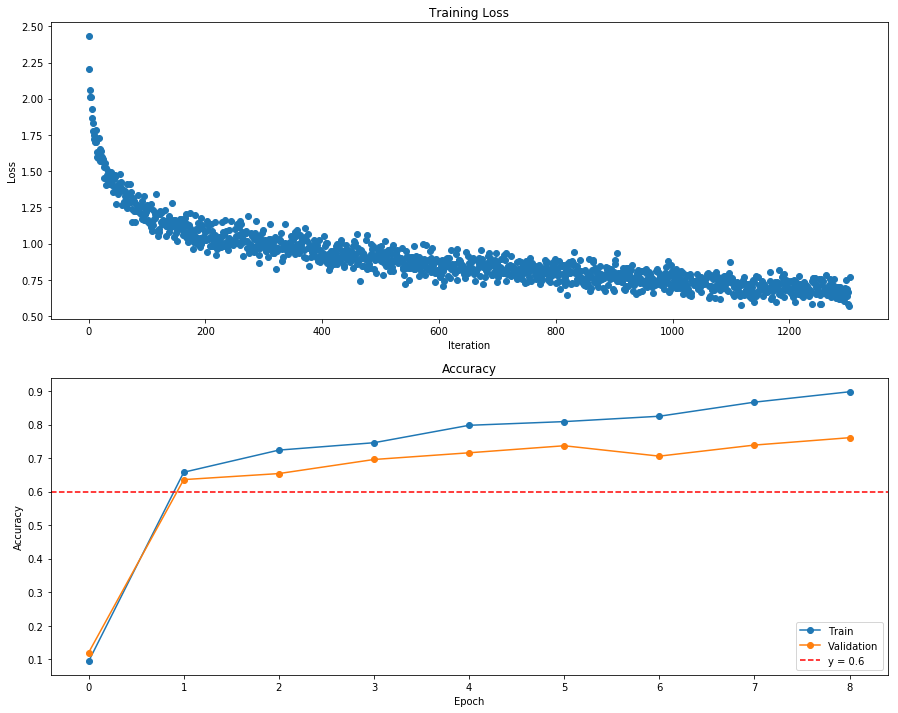
\includegraphics[width=0.8\textwidth]{image/Train your best model.png}
\end{figure}

在训练过程中，训练损失随迭代推进持续下降，说明卷积特征提取与全连接分类头能够稳定参与优化，模型已经学到数据中的有效判别信息。

从准确率曲线来看，训练准确率在后期保持上升，而验证准确率在达到较高水平后趋于平台并出现轻微回落。这表明该网络在 CIFAR-10 上已经具备较好的表达能力，同时也存在一定程度的过拟合倾向。

在本次作业中，最终验证准确率为 \underline{0.7390}（已在训练日志中展示）。